% !TeX TS-program = xelatex


\documentclass[aspectratio=169,13pt,fleqn,t] {beamer}
%
% Choose how your presentation looks.
%
% For more themes, color themes and font themes, see:
% http://deic.uab.es/~iblanes/beamer_gallery/index_by_theme.html
%
\mode<presentation>
{
	\usetheme{Madrid}      % 整体主题
	\usecolortheme{beaver} % 配色主题（棕红系）
	\usefonttheme{serif}   % 全局衬线字体（正文宋体类）
	\setbeamertemplate{items}[default] % 【items父模板】控制 itemize+enumerate 符号
%	\setbeamertemplate{items}{\Large\beamertemplateballitem}
	\setbeamertemplate{sections/subsections in toc}[ball] % 目录里章节用圆圈标记
	
	%  \setbeamertemplate{navigation symbols}{} % 取消注释可隐藏底部导航小图标
	\setbeamertemplate{caption}[numbered] % 图/表标题带编号：图1、表1
}

\usepackage[,UTF8,linespread=1.2]{ctex}
\usepackage{wrapfig}
\usepackage{caption}
\usepackage{tcolorbox}
\tcbuselibrary{skins}
\captionsetup[figure]{name=图,labelsep=period}
\usepackage{pdfpages}
\usepackage{tabularx,array}
\usetikzlibrary{arrows.meta,intersections,positioning}


\usepackage{xcolor}
\definecolor{xy_blue}{cmyk}{0.6,0.35,0.0,0.4}
\definecolor{xy_orange}{cmyk}{0.0,0.7,1.0,0.0}
\definecolor{xy_green}{cmyk}{0.2,0.0,1.0,0.15}
\xdefinecolor{xy_gold}{RGB}{135,103,79}
\xdefinecolor{xy2_gold}{cmyk}{0,0.35,0.75,0.05}

\setbeamercolor{section number projected}{fg=red,bg=red!20}%控制球的颜色
\setbeamercolor{subsection number projected}{fg=blue,bg=blue!40}
\setbeamercolor{item}{fg=xy_gold} %设置列表项颜色

\usepackage{amsthm}
\newtheorem{peroration}{结论：}
\newtheorem*{exploration}{探究：}
\newtheorem*{prooft}{证明：}
\newtheorem*{solve}{解:} 
\newtheorem{instance}{例}   % 解：独立计数器
\newtheorem*{definate}{定义：}
     

% 配色（你前面需要的，每个环境单独颜色）
\setbeamercolor{theorem}{fg=black,bg=blue!10}
\setbeamercolor{solution}{fg=black,bg=green!10}

\BeforeBeginEnvironment{peroration}{%结论： 
	\setbeamercolor{block title}{bg=xy_green,fg=white}
	\setbeamercolor{block body}{bg=xy_green!10}
}
\AfterEndEnvironment{peroration}{
	\setbeamercolor{block title}{bg=xy_blue,fg=white}
	\setbeamercolor{block body}{bg=xy_blue!10}
}
\BeforeBeginEnvironment{exploration}{%探究
	\setbeamercolor{block title}{bg=xy_orange,fg=white}
	\setbeamercolor{block body}{bg=xy_orange!10}
}
\AfterEndEnvironment{peroration}{
	\setbeamercolor{block title}{bg=xy_blue,fg=white}
	\setbeamercolor{block body}{bg=xy_blue!10}
}
\BeforeBeginEnvironment{solution}{%解
	\begingroup
	\setbeamercolor{block title}{bg=xy_green,fg=white}
	\setbeamercolor{block body}{bg=xy_green!10}
}
\AfterEndEnvironment{solution}{
	\endgroup
}
\BeforeBeginEnvironment{prooft}{%证明
	\setbeamercolor{block title}{bg=xy_green,fg=white}
	\setbeamercolor{block body}{bg=xy_green!10}
}
\AfterEndEnvironment{prooft}{
	\setbeamercolor{block title}{bg=xy_green,fg=white}
	\setbeamercolor{block body}{bg=xy_green!10}
}
\BeforeBeginEnvironment{solve}{%解：
	\setbeamercolor{block title}{bg=xy_orange!60,fg=white}
	\setbeamercolor{block body}{bg=xy_orange!10}
}
\AfterEndEnvironment{solve}{%解：
	\setbeamercolor{block title}{bg=xy_orange!60,fg=white}
	\setbeamercolor{block body}{bg=xy_orange!10}
}
   
\BeforeBeginEnvironment{instance}{% 例子
	\begingroup
   	\setbeamercolor{block title}{bg=xy_gold!40,fg=white}
   	\setbeamercolor{block body}{bg=xy_gold!10}
   }
\AfterEndEnvironment{instance}{
	\endgroup
   }     
   
\renewcommand{\thefigure}{\arabic{figure}}

\title[2.3~一元二次不等式]{2.3~~二次函数与一元二次方程、不等式}
\author[好好学习，努力向上]{}
\institute{}
\date{2026.9.28}
\setbeamertemplate{theorems}[numbered]

\AtBeginSection[]
{
  \begin{frame}<beamer>
    \frametitle{本节主要内容}
    \tableofcontents[currentsection,currentsubsection]
  \end{frame}
}

\begin{document}
\begin{frame}{}
	\titlepage
\end{frame}

\begin{frame}{内容概览}
	\tableofcontents
\end{frame}

\section{前情回顾}
\begin{frame}{前情回顾}
	
	\begin{enumerate}
		\item 一元二次方程：形如$ax^2+bx+c=0(a\neq 0)$这样的方程叫做一元二次方程。
		\begin{enumerate}[(1)]
			\item 求根公式$x_{1,2}=\frac{-b\pm \sqrt{b^2-4ac}}{2a}$.
			\item 韦达定理：$x_1+x_2=-\frac{b}{a},x_1x_2=\frac{c}{a}$.
		\end{enumerate}
		\item 二次函数：形如$y=ax^2 + bx + c(a\neq 0)$这样的函数叫做二次函数。
		\begin{enumerate}[(1)]
			\item 二次函数的图象是抛物线；
			\item 开口方向由$a$确定，$a>0$时，开口向上，$a<0$时开口向下；
			\item 图象与$x$轴的交点情况由$\Delta$确定：$\Delta>0$时有两个交点，$\Delta=0$时有一个交点，
			$\Delta<0$时没有交点。
			\item 二次函数图象的对称轴：$x=-\frac{b}{2a}$；
			\item 二次函数的最值情况：$a>0$时，有最小值$\frac{4ac-b^2}{4a}$，$a<0$时有最大值$\frac{4ac-b^2}{4a}$。
		\end{enumerate}
	\end{enumerate}
	
\end{frame}

\section{一元二次不等式及其解法}
\begin{frame}[t]{一元二次不等式的概念}
	\begin{definate}[一元二次不等式]
		我们把只含有一个未知数，并且未知数的最高次数是$2$的不等式，称为\textbf{一元二次不等式}，它的一般形式为
		\[
		ax^2+bx+c>0,\text{或}\quad ax^2+bx+c<0
		\]
		其中$a$，$b$，$c$均为常数，$a\neq 0$.
	\end{definate}
	
	
\end{frame}

\begin{frame}[t]{一元二次不等式与二次函数、一元二次方程的关系}
\begin{definate}[二次函数的零点]
	一般地，对于二次函数$y=ax^2+bx+c$，我们把使$ax^2+bx+c=0$的实数$x$叫做二次函数$y=ax^2+bx+c$的零点。
	
	因此，二次函数的零点就是相应一元二次方程的根。
\end{definate}

\end{frame}


\begin{frame}[t]{一元二次不等式与二次函数、一元二次方程的关系}
	\small
	\begin{tabularx}{\textwidth}[c]{|*{4}{>{\arraybackslash}m{3.37cm}|}}
		\hline
		\centering 项目 &	\centering $\Delta>0$	& \centering$\Delta=0$	&	\centering\arraybackslash$\Delta<0$	\\
		\hline
		$y=ax^2+bx+c(a>0)$的图象	&	
		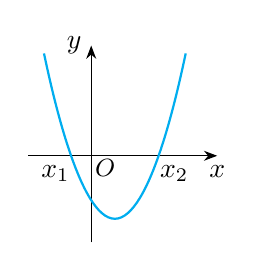
\begin{tikzpicture}[baseline={(0,-1)}]
			\draw[-Stealth,name path=line](-0.8,0) -- (1.6,0)node[below]{$x$};
			\draw[-Stealth](0,-1.1) -- (0,1.4)node[left]{$y$};
			\draw[thick,cyan,name path=curve](-0.6,1.3) parabola bend(0.3,-0.8) (1.2,1.3);
			\path[name intersections={of= line and curve,name=t}]
			(t-1)node[below left= 0pt and  -3pt]{$x_1$}
			(t-2)node[below right= 0pt and  -3pt]{$x_2$};
			\node[below right=-3pt] at (0,0){\small $O$};
		\end{tikzpicture}	&	
		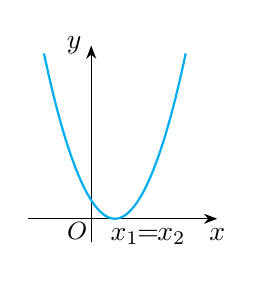
\begin{tikzpicture}[baseline={(0,-1)}]
			\draw[-Stealth,name path=line](-0.8,-0.8) -- (1.6,-0.8)node[below]{$x$};
			\draw[-Stealth](0,-1.1) -- (0,1.4)node[left]{$y$};
			\draw[thick,cyan,name path=curve](-0.6,1.3) parabola bend(0.3,-0.8) (1.2,1.3);
			\path[name intersections={of= line and curve,name=t}]
			(t-1)node[below right =0pt and -5pt ]{$x_1\!\!=\!\! x_2$};
			\node[below left=-3pt] at(0,-0.8){\small $O$};			
		\end{tikzpicture}		&	
		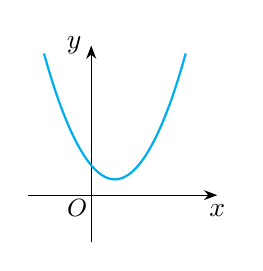
\begin{tikzpicture}[baseline={(0,-1)}]
			\draw[-Stealth,name path=line](-0.8,-0.5) -- (1.6,-0.5)node[below]{$x$};
			\draw[-Stealth](0,-1.1) -- (0,1.4)node[left]{$y$};
			\draw[thick,cyan,name path=curve](-0.6,1.3) parabola bend(0.3,-0.3) (1.2,1.3);			
			\node[below left=-3pt] at(0,-0.5){\small $O$};			
		\end{tikzpicture}	\\
		\hline
		$ax^2+bx+c=0(a>0)$的根	&	有两个不相等的实数根$x_1,x_2(x_1<x_2)$	&	有两个相等的实数根$x_1=x_2=-\frac{b}{2a}$	&	没有实数根	\\
		\hline
		$ax^2+bx+c>0(a\neq 0)$的根	&$\{x\mid x<x_1,\text{或} x>x_2\}$	&	$\{x\mid x \neq -\frac{b}{2a}\}$	&	\centering\arraybackslash$\mathbf{R}$		\\
		\hline
		$ax^2+bx+c<0(a>0)$的解集	&	\centering$\{x \mid x_1<x<x_2\}$		&	\centering$\varnothing$	&	\centering\arraybackslash$\varnothing$	\\
		\hline
	\end{tabularx}
%\vspace{-2em}
%\begin{figure}
%	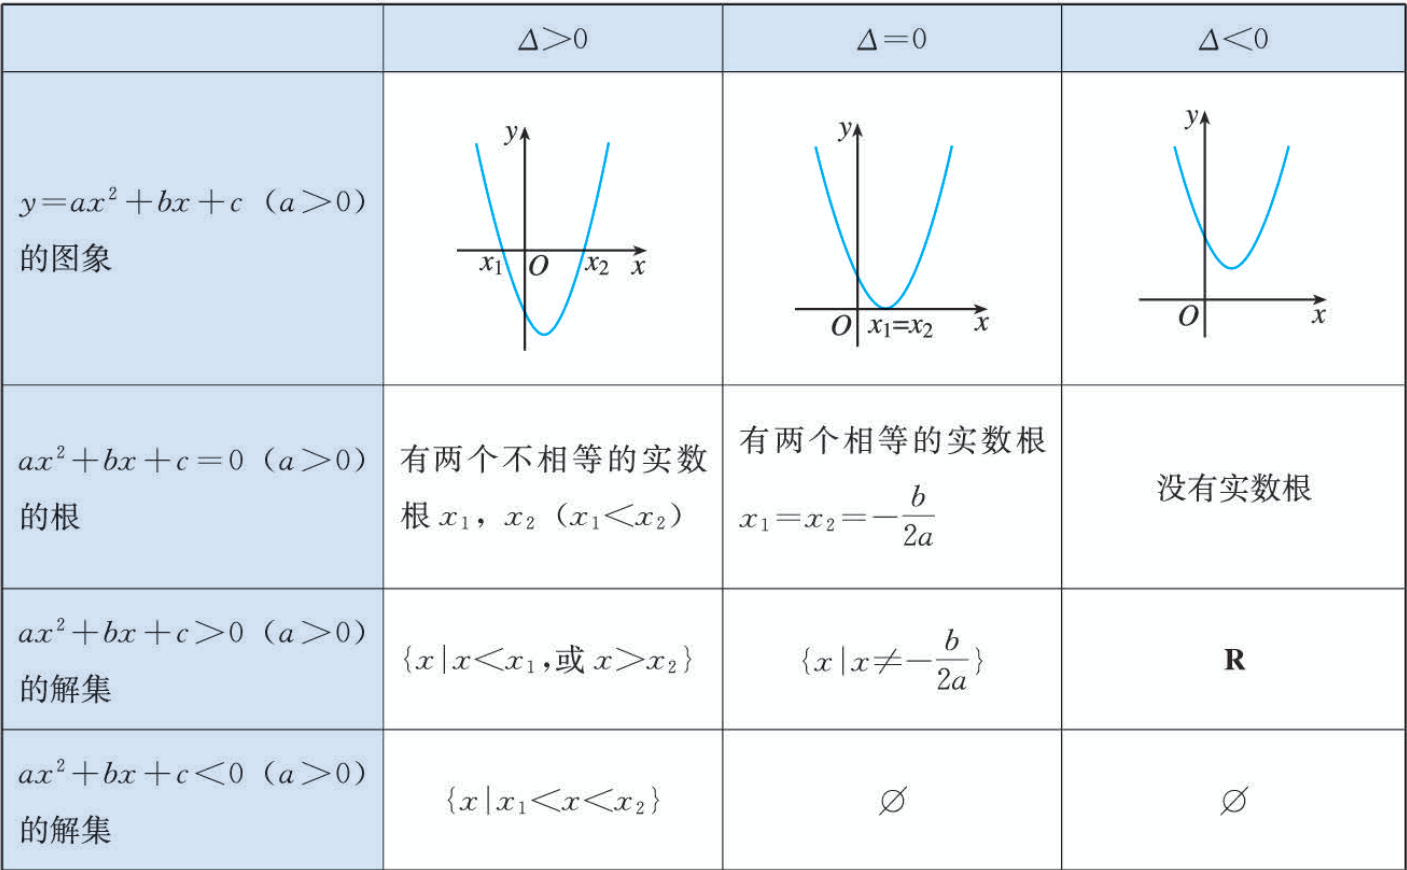
\includegraphics[height=7.5cm]{Figures/budengshi.png}
%\end{figure}

\end{frame}

\begin{frame}[<+->]{例题分析}
	\vspace{-1.5em}
\begin{instance}
	求不等式$x^2-5x+6>0$的解集。
\end{instance}
\vspace{-1em}
\begin{solve}
	
	\begin{wrapfigure}{r}{4cm}
	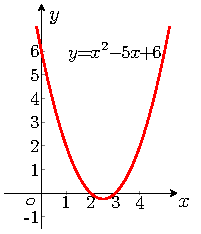
\includegraphics[,height=4.5cm]{Figures/budengshi4.pdf}
	\end{wrapfigure}
	解方程$x^2-5x+6=0$得$x_1=2,x_2=3$，
	
	结合函数$y=x^2-5x+6$的图像，
	
	可得不等式的解集为
	$\{x| x<2,\text{或} \;x>3\}$。
	
	\vspace{7.5em}
	~
	

	
\end{solve}
\end{frame}

\begin{frame}[<+->]{例题分析}
	\vspace{-1.5em}
	\begin{instance}
		求不等式$9x^2-6x+1>0$的解集。
	\end{instance}
	\vspace{-1em}
	\begin{solve}		
		\begin{wrapfigure}{r}{4.5cm}
			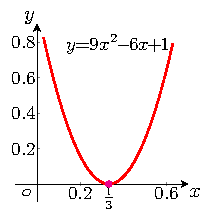
\includegraphics[,height=4.5cm]{Figures/budengshi5.pdf}
		\end{wrapfigure}
		对于方程$9x^2-6x+1=0$，因为$\Delta=0$，所以它有两个相等的实数根。解得$x_1=x_2=\frac{1}{3}$.
		
		画出函数$y=9x^2-6x+1$的图象，
		
		结合函数$y=9x^2-6x+1$的图像，
		
		可得不等式的解集为
		$\{x| x\neq \frac{1}{3}\}$。
		
		\vspace{5em}
		~
	\end{solve}
\end{frame}

\begin{frame}[<+->]{例题分析}
	\vspace{-1.5em}
	\begin{instance}
		求不等式$-x^2+2x-3>0$的解集。
	\end{instance}
	\vspace{-1em}
	\begin{solve}		
		\begin{wrapfigure}{r}{4.5cm}
			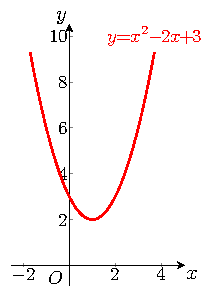
\includegraphics[,height=4.5cm]{Figures/budengshi6.pdf}
		\end{wrapfigure}
		不等式可化为$x^2-2x+3<0$。
		
		
		因为$\Delta=-8<0$，所以方程$x^2-2x+3=0$无实数根。
		
				
		画出函数$y=x^2-2x+3$的图象，
		
		结合函数$y=x^2-2x+3$的图像，
		
		可得不等式的解集为$\varnothing$。
		
		因此不等式的解集为$\varnothing$。
		
		
		\vspace{3.2em}
		~
	\end{solve}
\end{frame}

\begin{frame}{小结：解一元二次不等式的步骤}
	\vspace{-1em}
	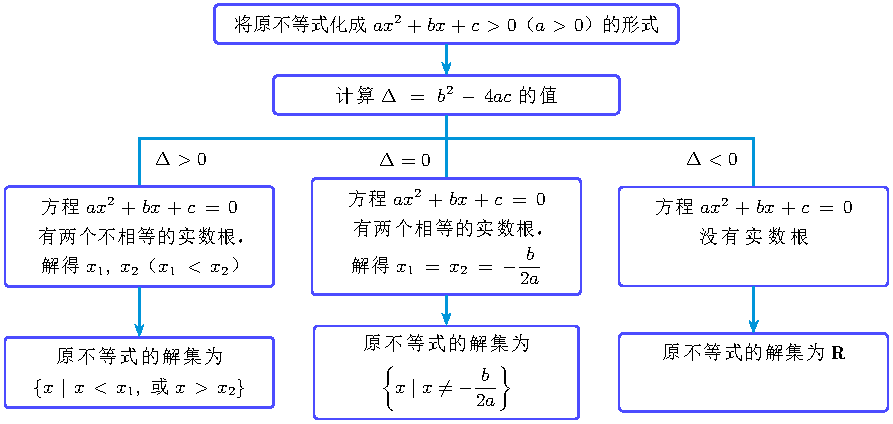
\includegraphics{Figures/budengshi7.pdf}
\end{frame}

\begin{frame}[t]{布置作业}
	
	P53 练习 ：1,2

	P55 习题2.3：1,2,3,5

\end{frame}

\end{document}
